%----------------------------------------------------------------------------
\chapter*{Zynq SoC}\addcontentsline{toc}{chapter}{Zynq SoC}
%----------------------------------------------------------------------------

\begin{figure}[!ht]
	\centering
	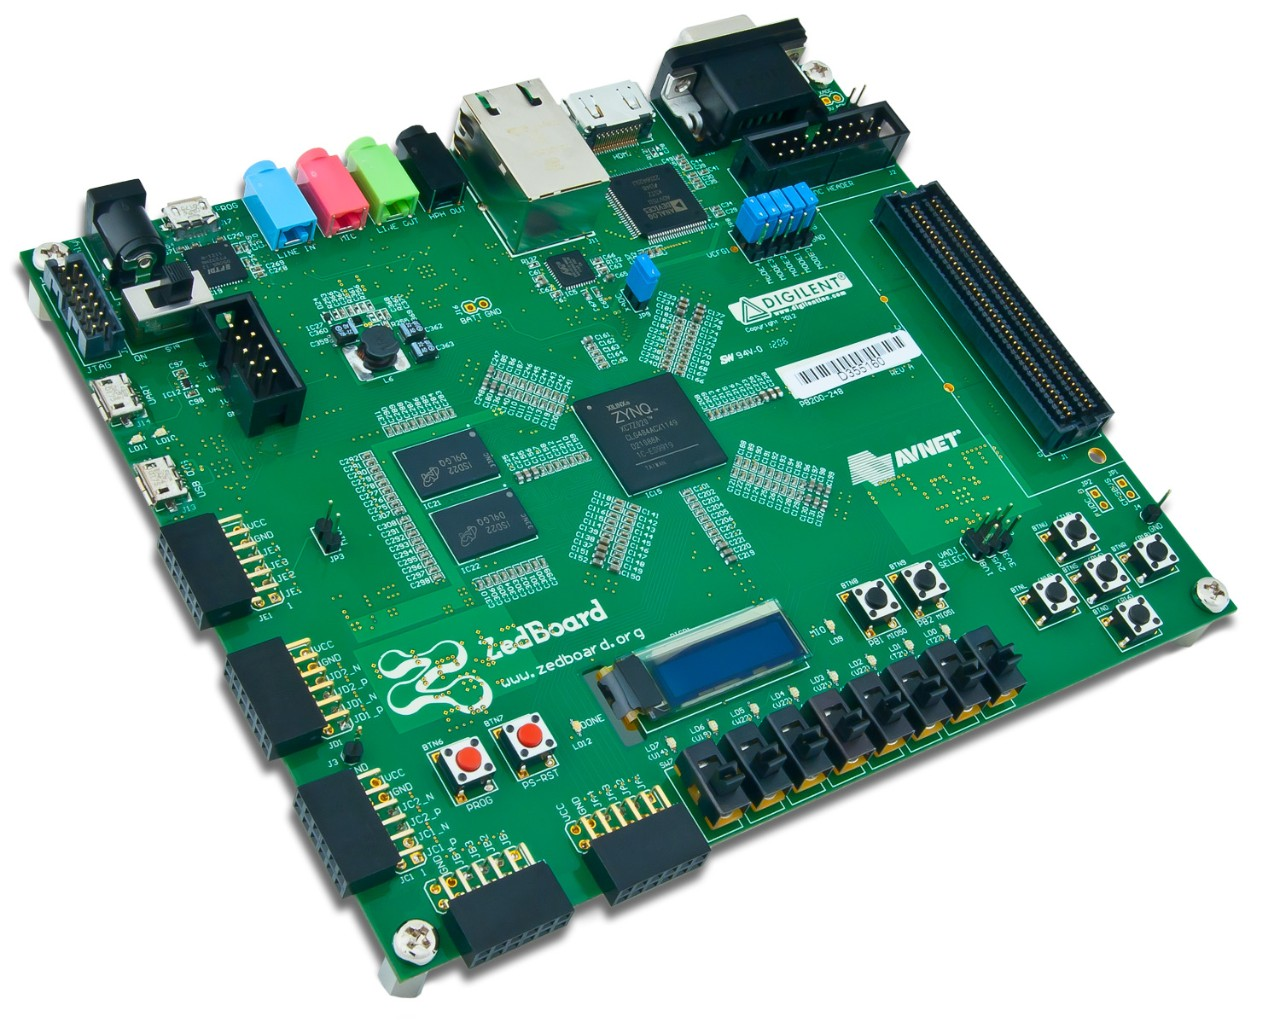
\includegraphics[width = \textwidth]{figures/1381869368208.jpg}
	\caption{A munka során használt ZedBoard} 
	\label{fig:zedboard}
\end{figure}

\begin{figure}[!ht]
	\centering
	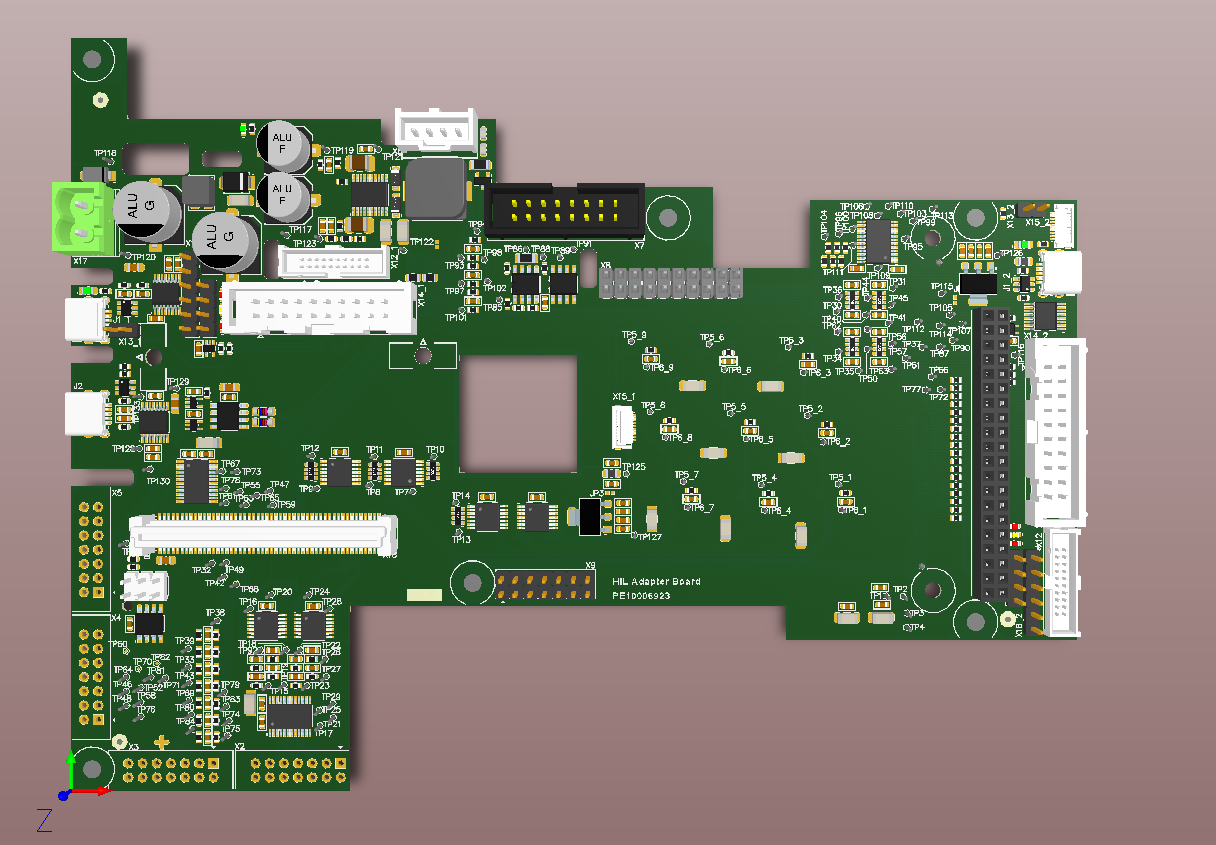
\includegraphics[width = \textwidth]{figures/kieg_nyak.png}
	\caption{A Hyundai által fejelsztett kiegészítő elektornika} 
	\label{fig:kiegnyak}
\end{figure}

\begin{figure}[!ht]
	\centering
	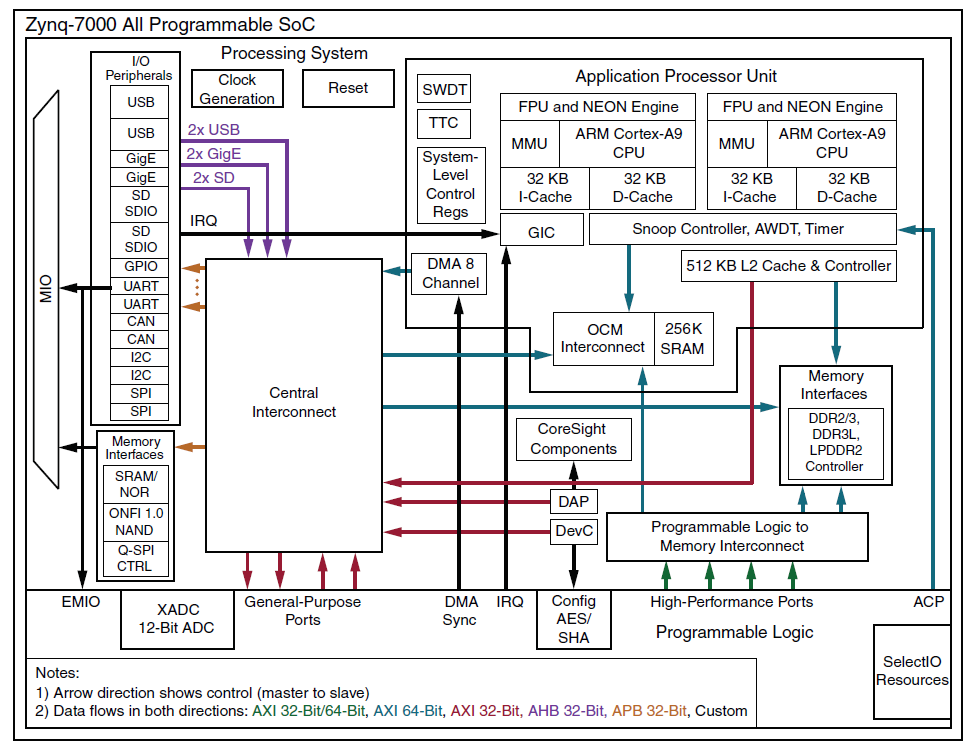
\includegraphics[width = \textwidth]{figures/socfelepites.png}
	\caption{A Xilinx Zynq Z-7000 SoC felépítése\cite{ZynqSOC}} 
	\label{fig:z7000}
\end{figure}